\chapter{Research}
This chapter is composed of three sections. The first concerns itself with existing research within the area of the analysis of social networks. The second . The final section is concerned with distributed computing, and how it can be used for analysing graphs of social networks.

% Since we have a few distinct sections on this area, I think it's a good idea to split this into multiple smaller files as well

\section{Social Network Analysis}
Analysis of social networks is becoming ever-increasing in importance, with the huge growth social network sites such as Facebook\footnote{\url{https://www.facebook.com/}} and Twitter\footnote{\url{http://twitter.com/}} have experienced in recent years. This research undertaken within this section relates to various metrics which can be applied to a social network to identify important people within the network, and also how the structure of the network can be identified.

\subsection{Community Detection}
An important aspect of social network analysis is the detection of communities within a graph. The identifying of communities within a social network can help to identify group dynamics of the network. 

A famous example of this is the friendship network within Zachary's karate club \cite{zachary77}, which subsequently split into the two groups shown in Figure \ref{fig:karate}. The identification of two clusters, which cleanly divided the network into the two groups the karate club actually split into, shows the usefulness of being able to identify connections between groups of highly interlinked individuals.

\begin{figure}%
\centering
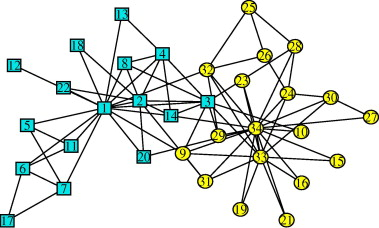
\includegraphics[width=0.5\columnwidth]{./img/karate}%
\caption{Clusters found within Zachary's karate club \cite{zachary77,comellas10}}%
\label{fig:karate}%
\end{figure}

\subsubsection{Clustering}
Within social networks, there are distinct regions of vertices with many connections passing between them, and a much smaller number connected to other vertices outside of this region. These regions are termed as \emph{clusters}.

Social networks are a prime example of this. A person tends to have groups of friends distinct from each other, and friends within these groups are also friends of each other. Figure \ref{fig:socialnetwork} is a social network constructed from data regarding mutual friends of a person. Within this Figure, it can clearly be seen that there exists five distinct regions of mutual friends, with very few links between these regions. These regions are the clusters described above.

With data presented in this manner, it is clear to an observer where these clusters exist, and how many distinct clusters there are. \cite{girvan02} presents an approach to identifying communities within a graph.

\begin{figure}[htbp]
\centering
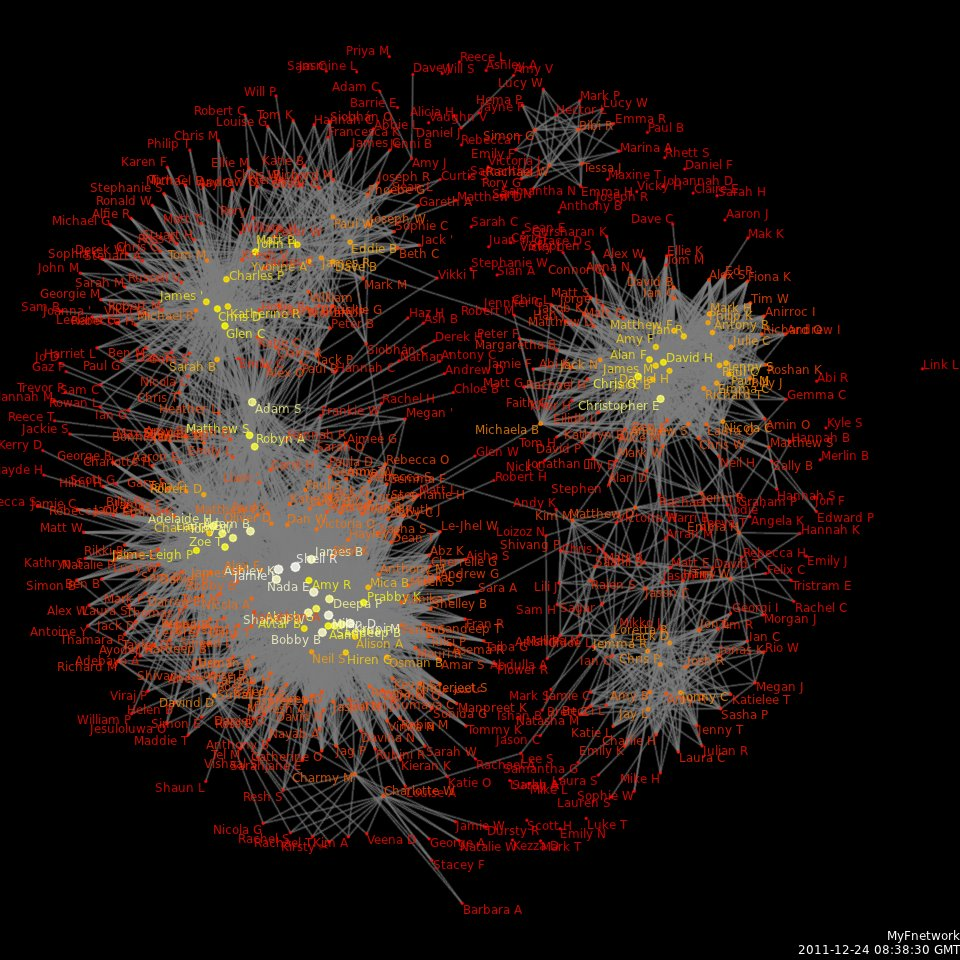
\includegraphics[width=0.5\textwidth]{./img/socialnetwork.png}
\caption{Social Network constructed from Facebook friends using the myFnetwork app}
\label{fig:socialnetwork}
\end{figure}

\subsubsection{Partitioning}
Partitioning of a graph differs from clustering slightly. To partition a graph, we first must know the number of partitions we wish to make, and also the size of each of these partitions. Clustering does not need to know this information as the clusters are produced by the algorithms performing the clustering. Partitioning is related to clustering as it splits the input graph into distinct smaller subgraphs of highly connected vertices, with the subgraphs representing communities within the original graph.

The process of graph partitioning is to divide a graph into smaller parts, such that the number of connections between these smaller parts is as few as possible. The partitions produced are non-overlapping, of a given size, and of a given number.

Graph partitioning is known to be a difficult and complex problem to solve. For simplicity, assume that we are to partition a graph into two partitions. To naively \emph{brute force} all permutations to find the ``best'' partition, which minimises the number of connections between the two partitions, soon becomes unfeasible for anything but the smallest graphs, due to the number of ways of partitioning \emph{n} verticies into two groups \emph{$n_1$} and \emph{$n_2$}. This is $\frac{n!}{n_1!n_2!}$ permutations, and with application of Stirling's formula, can we rewritten as \cite{newman10}:

\begin{equation}
\frac{n!}{n_1!n_2!} \simeq \frac{\sqrt{2\pi n}(n/e)^n}{\sqrt{2\pi n_1}(n_1/e)^{n_1} \sqrt{2\pi n_2}(n_2/e)^{n_2}} = \frac{n^{n+1/2}}{n_1^{n_1+1/2} n_2^{n_2+1/2}} 
\label{eq:partioning1}
\end{equation}

Which, if our two partitions $n_1$ and $n_2$ are equal in size, then the number of permutations of the partition is \cite{newman10}:

\begin{equation}
\frac{n^{n+1/2}}{(n.2)^{n+1}} = \frac{2^{n+1}}{\sqrt{n}}
\label{eq:}
\end{equation}

This shows that running time of the \emph{brute force} algorithm to find all permutations grows exponentially with the size of the input graph.

\citeauthor{kernighan70} proposed an algorithm to solve the partitioning of a graph into two sections \cite{kernighan70}. Initially, the graph is split into two partitions, \emph{A} and \emph{B}. For each pair of vertices (\emph{i, j}) such that $i \in A$ and $j \in B$, the algorithm finds the pair which reduces the number of connections between \emph{A} and \emph{B} the most (see Figure \ref{fig:kernighanlin1}), and swap them (Figure \ref{fig:kernighanlin2}). If there is no pair which reduces the number of connections between the two partitions, then the pair which increases the number of connections by the smallest amount are swapped. This is then repeated until vertices within one partition have been swapped, with the condition that once a vertex has been swapped, it cannot be swapped again. Following this, each state the graph was in after a swap is revisited, with the state with the minimum number of connections between \emph{A} and \emph{B} is minimal. These steps are then repeated until \emph{A} and \emph{B} do not change between rounds. The algorithm has been shown to run in $O(n^2\: log\: n)$ time \cite{kernighan70}, which is marked improvement over the \emph{brute force} $O(2^n)$, but still remains slow and unsuitable for graphs with a over a few thousand vertices \cite{newman10}.

\begin{figure}[htbp]
  \centering
  \subfloat[Original network]{\label{fig:kernighanlin1}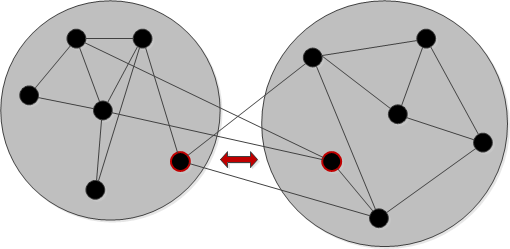
\includegraphics[width=0.3\textwidth]{./img/kernighanlin1}}
  ~ 
  \subfloat[The same network after interchange of two vertices]{\label{fig:kernighanlin2}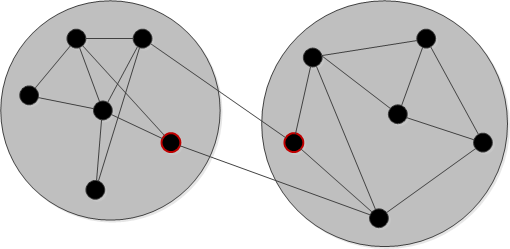
\includegraphics[width=0.3\textwidth]{./img/kernighanlin2}}
  ~ 
  \caption{The Kernighan-Lin algorithm \cite{newman10}}
  \label{fig:kernighanlin}
\end{figure}

Figure \ref{fig:kernighanlin} shows the effect of the Kernigham-Lin algorithm on the original network (Figure \ref{fig:kernighanlin1}). The two vertices highlighted with red reduce the number of connections between the two groups the most, so are swapped. This swap is also the best swap which happens during this iteration of the algorithm, so the network in Figure \ref{fig:kernighanlin2} is selected as the initial network for the next iteration. As no vertex swapping can improve on this, and as such this network is the best network for the next iteration, this network is the solution from the algorithm and the algorithm terminates.

To split a graph into more than two partitions, repeated application of partitioning the subgraphs produced from previous partitioning is applied.

There exist other algorithms to partition graphs, notably spectral algorithms \cite{pothen90,fiedler73}, which make use of properties of the matrix which can be used to define a graph. These spectral algorithms are a lot more complex in the operations needed to execute them, however they operate in $O(n^2)$ time, which is an order $n$ faster than the Kernighan-Lin algorithm \cite{newman10}. It is also noted that spectral algorithms do not necessarily give the best partition, with the partitions produced being of the rough general shape but not quite as good as other algorithms \cite{newman10}.

\subsubsection{\emph{k}-Cliques}
The term \emph{clique} is introduced by \citeauthor{luce49} in \cite{luce49} to describe a subgraph which consists of at least three vertices, each of which are fully connected with each other. From a social network perspective, this translates to saying that for each person in the clique, all of their friends  within the clique are friends of each other as well.

A \emph{k}-clique is defined as a clique which has size \emph{k}. A \emph{maximal clique} is a clique to which no more vertices can be added without violating the conditions of a clique, and the maximum clique is a clique within a graph which contains the largest number of vertices. A 3-clique is also known as a triangle, due to the shape of the graph they are normally represented as (Figure \ref{fig:3clique}).

\begin{figure}[htbp]
\centering
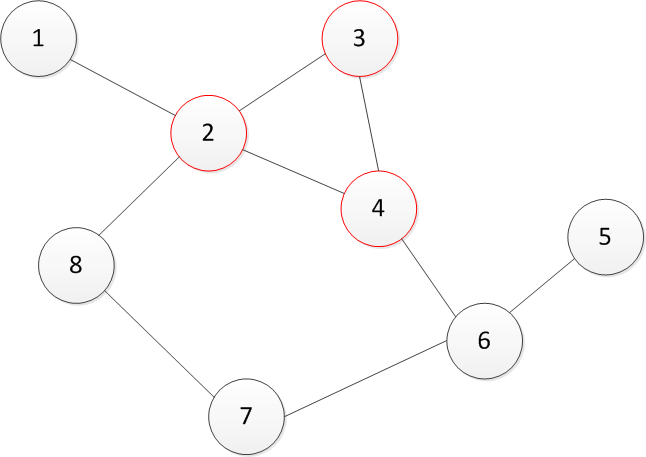
\includegraphics[width=0.5\textwidth]{./img/clique.png}
\caption{Graph highlighting a 3-clique}
\label{fig:clique}
\end{figure}

Figure \ref{fig:clique} shows an example graph highlighting a 3-clique. It has one maximum clique \{2,3,4\} which is highlighted in red, and six other maximal cliques \{1,2\}, \{2,8\}, \{4,6\}, \{5,6\}, \{6,7\}, \{7,8\}.

\begin{figure}
  \centering
  \subfloat[3-clique]{\label{fig:3clique}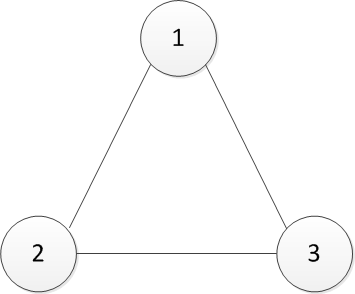
\includegraphics[width=0.3\textwidth]{./img/3-clique}} ~ \subfloat[4-clique]{\label{fig:4clique}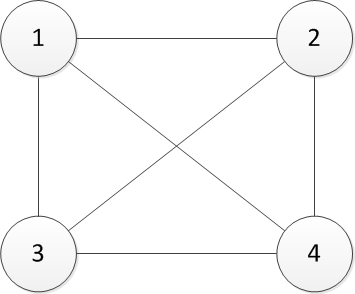
\includegraphics[width=0.3\textwidth]{./img/4-clique}} ~ \subfloat[5-clique]{\label{fig:5clique}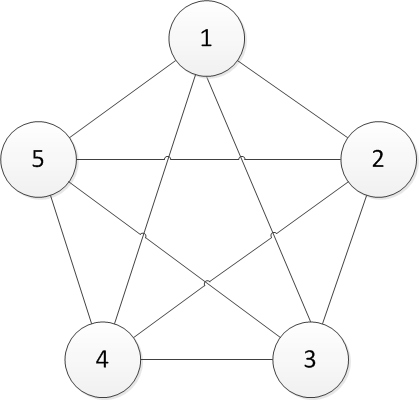
\includegraphics[width=0.3\textwidth]{./img/5-clique}}
  \caption{\emph{k}-cliques}
  \label{fig:cliques}
\end{figure}

Identifying cliques, and solving problems involving cliques as been shown to be computationally hard \cite{bomze99, trusses}. Cliques are either too common, with cliques of only a few members are frequently too numerous to be helpful, or too rare, with large cliques too limiting to be of use \cite{trusses}. Also, computation of identifying cliques scales worse than any polynomial of the problem size, making the process unfeasible for large graphs \cite{trusses, bron72}.

There have been numerous generalisations of the clique construct to improve usefulness of the clique through relaxation of some of the properties of the clique. These include the \emph{n}-clique \cite{luce50}, \emph{n}-clan \cite{alba73} and \emph{n}-club \cite{mokken79}. However these new constructs do not solve the issues of identifying cliques, and remain hard to compute and produce too many results.

\subsubsection{\emph{k}-Trusses}
Following from relaxing properties of the clique, \citeauthor{trusses} in \cite{trusses} introduces a new construct called a truss. A \emph{k}-truss is a subgraph where an edge between two vertices, A and B, exists if at least \emph{k-2} other vertices are connected to both of A and B. The \emph{k}-truss has similar definitions to the clique. A maximal \emph{k}-truss is a \emph{k}-truss that is not a proper subgraph of another \emph{k}-truss.

\begin{figure}[htbp]
\centering
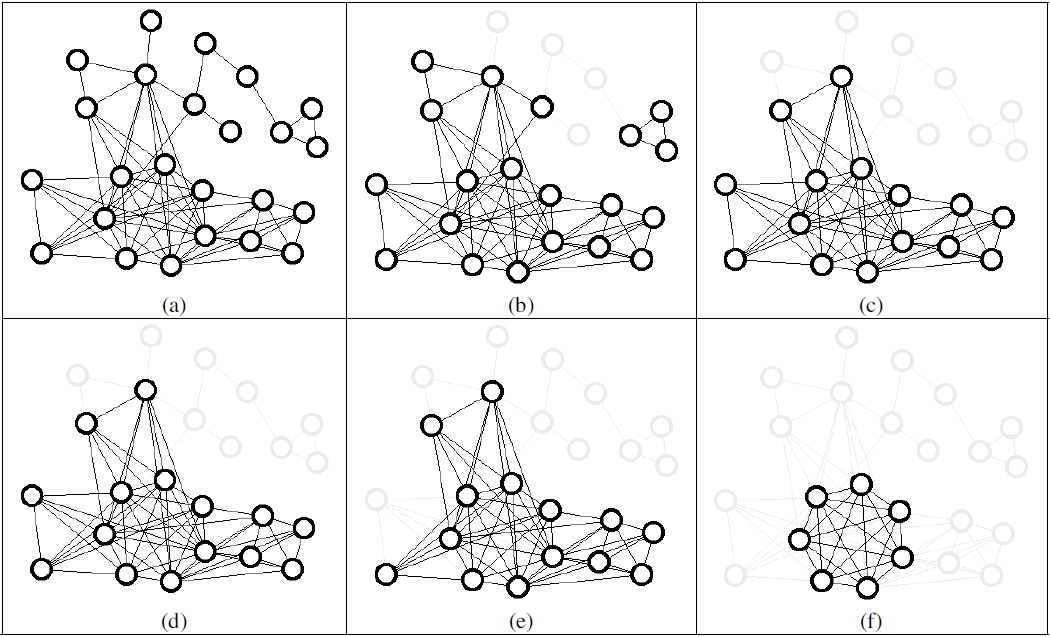
\includegraphics[width=0.9\textwidth]{./img/trusses.png}
\caption{An Example of Maximal Trusses. (a) original graph, (b) 3-trusses, (c) 4-truss, (d) 5-truss, (e) 6-truss. Note that (c) and (d) are the same. \cite{trusses}}
\label{fig:trusses}
\end{figure}

Figure \ref{fig:trusses} shows an example application of \emph{k}-trusses. Figure \ref{fig:trusses}(a) shows the original graph. Figures \ref{fig:trusses}(b-f) show the \emph{k}-truss for increasing values of \emph{k}. If the same original graph were to be analysed for \emph{k}-cliques for the same values of \emph{k}, more vertices in the graph would have been removed in earlier stages, which would have lost the interesting stage where Figures \ref{fig:trusses}(c) and (d) are identical.

The \emph{k}-truss is also computable in polynomial time to the input graph, which offers a marked improvement on the computation costs of identifying cliques and similar constructs. \cite{trusses} shows that the naive algorithm  for computing maximal \emph{k}-trusses is bounded by $O(n|E|^2 + n)$, where \emph{n} is the number of vertices in the graph, and \emph{|E|} is the number of edges in the graph. A more efficient method is shown to take $O(\Sigma d^2(v))$, where \emph{d(v)} is the degree of a vertex, \emph{v}.

\subsection{Clustering Coefficients}
Clustering coefficients provide a way to measure the amount to which vertices within a graph cluster together. Calculating clustering coefficients requires knowing the number of triangles within the graph.

\subsubsection{Global Clustering Coefficient}
The global clustering coefficient is also known as the transitivity of a network. This is because it is similar to the mathematical property of transitivity. A relation ``$\circ$'' is said to be transitive if $a \circ b$ and $b \circ c$ imply together imply $a \circ c$. An example would be the equality relation, as if $a = b$, and $b = c$ it follows that $a = c$ \cite{newman10}. Within a social network, the transitive relation could be described as \textit{``the friend of my friend is also my friend''}.

A global clustering coefficient of 1 implies a social network where all components are cliques. A global clustering coefficient of 0 implies a social network where there are no mutual friends between any two people.

The global clustering coefficient is defined as:

\begin{equation}
C_G = \frac{3 * number\: of\: triangles}{number\: of\: connected\: triples}
\label{eq:globalcc}
\end{equation}

A connected triple is simply three vertices $uvw$ connected with edges ($u, v$) and ($v, w$); edge ($u, w$) does not need to be present \cite{newman10}. The factor 3 is present because each triangle is composed of three connected triples.

\subsubsection{Local Clustering Coefficient}
A clustering coefficient can also be applied to each vertex within a graph. The local clustering coefficient is the probability that vertices connected to a vertex are themselves also connected to each other.

The local clustering coefficient is defined as:

\begin{equation}
C_L = \frac{number\: of\: triangles\: connected\: to\: vertex\: v}{number\: of\: triples\: centered\: on\: vertex\: v}
\label{eq:localcc}
\end{equation}

Within social network analysis, the local clustering coefficient

\subsubsection{Network Local Clustering Coefficient}
The network local clustering coefficient is simply the mean of all local clustering coefficients within a network. It can be used to show the average level of connectedness between vertices in a network.

\begin{equation}
C_N = \frac{1}{n}\sum_{i=1}^{n} C_i
\label{eq:networkcc}
\end{equation}

$C_i$ represents the local clustering coefficient of the vertex $i$. The result of this calculation is a number between 0 and 1, with 1 meaning all vertices are connected to each other \cite{watts98}.

\subsection{Centrality}
Following from identifying communities within a social network, it is also apparent that establishing the most \emph{central} or \emph{important} person is within a community. This person is most likely going to have a large influence over the members of the community 

\subsubsection{}
\subsection{Influence Propogation}

 Influence propogation algorithms attempt to model the spread of ideas (Rogers 2003), viruses (Anderson and May 1991), word-of-mouth recommendations (Goldenberg, Libai and Muller 2001), viral marketing campaigns (Kempe, Kleinberg and Tardos 2003) or other transmissable entities, through a social network.

Influence propogation algorithms make the following assumptions about the social networks that they model. Social networks are modelled as directed graphs, with nodes representing individuals, and vertices representing relationships between individuals. In most influence propogation models, nodes can be in one of two states: "converted" or "unconverted". At the begin of the simulation, a subset of the nodes will be converted; over time they will convert their unconverted neighbours. There is an assumption of monotonicity, ie, converted nodes do not become unconverted.

 The exact conditions that determine when nodes will change from unconverted to converted depends on the influence propogation model used. There are three main models of transmission used; the independent cascade model, the linear threshold model, and ???

Mention more complicated models, three states etc

\subsubsection{Independent Cascade}
 In the independent cascade model, whenever a node becomes converted, it has one chance to convert each of its neighbours. Every edge (A -> B) is assigned a weight between 0 and 1, which represents the probability that node A can convert node B, or vice versa.

Assume a node n has a set of x neighbours n\_0,n\_1,n\_2...n\_x each with edge weights e\_0,e\_1,e\_2...e+x. When n is converted, each neighbour n\_m has a e\_m chance to become converted.

This can be expressed in pseudocode as follows:

recently-converted-nodes = a queue of the initially converted nodes
while recently-converted-nodes is non-empty {
  node = recently-converted-nodes.next()
  for each neighbour in node.neighbours {
    if rand(0,1) < neighbour.edge-weight {
      neighbour.converted = true
      recently-converted-nodes.enqueue(neighbour)
    }
  }
}

\subsubsection{Linear Threshold}
 In the linear threshold model, every node has a threshold value t. When the number of converted neighbours is greater than t, the node becomes converted. Again, edges can be weighted, in which case the condition for conversion is:

Maths: sum for all neighbours(if neighbour is converted(0,1) * edge weight)

That is, nodes are converted when a threshold of their neighbours are converted. In pseudocode:

do {
  changed-nodes = 0
  for each node in unconverted-nodes {
    neighbour-influence = 0
    for each neighbour in neighbours {
      if neighbour.converted {
        neighbour-influence += neighbour.edge-weight
      }
    }
    if neighbour-influence >= node.threshold {
      node.converted = true
      changed-nodes += 1
    } 
  }
} while changed-nodes > 0

\subsubsection{Decreasing Cascade Model}


\subsubsection{Influence Maximisation Problem}

[Maximizing the Spread of Influence through a Social Network]

[http://arxiv.org/pdf/math/0612046.pdf]

One common use of an influence propogation model is to determine the best subset of nodes, that, if converted at the start of the simulation, will maximise the number of converted nodes at the end of the simulation. More formally, given a fixed budget k, and a function f(S), which takes an initial set of converted nodes and computes the expected final number of converted nodes, find a set of k nodes that maximises f(S).

One practical example would be a viral marketing company that might wish to kickstart their campaign by giving a group of influential bloggers a free trial of their service, and hope that these bloggers would then hopefuly recommend the product to their followers, who would recommend it to their followers, and so on. One strategy for choosing the optimal set of free trial users would be to rank the bloggers by a precomputed influence rating, and then select the top k most influential individuals from the list.

Even if influence of a single node could be computed reliably, this strategy would not generally find the optimum subset. For example, the most influential bloggers might share the same audience, wheras a less popular blogger might have considerable influence amongst a niche audience. In graph theory terms, there may be a short distance between two influential nodes -- they may even share overlapping neighbourhoods -- which means there may be a set of nodes far from the influential pair. These nodes might be more influenced by a node that is less globally influential, but nearer. Obviously, the structure of the graph determines the likelihood of this. For example, graphs with a community structure are more likely to require an influential seed node within each community to achieve maximum influence.

Solving the optimum problem is NP-hard, for both the linear threshold and independent cascade models. This can be shown by reducing the independent cascade maxmisation problem to a special case of the set cover problem, and the linear threshold maximisation problem to a special case of the vertex cover problem.

However, a greedy solution works as an approximation. !he set of nodes chosen by the greedy solution will convert at least 63\% of the nodes converted by the optimum solution. This result can be proved by showing that the function f(S) is monotonic and submodular.

The monotonicity property requires that f(S) increases whenever an element is added to S; ie, f(S+v) >= f(S) for any S, v. Proving this property of f(S) is trivial. The submodularity property can be intuitively thought of as a ``dimininishing returns'' property; if S is a subset of T, the marginal gain from adding an element v to S is at least as high as adding the same element to T. Formally:

f(S+v) - f(S) >= f(T+v) - f(T)

Nemhauser, Wolsey and Fisher showed that a greedy-hill climbing algorithm can be used to find the optimum value of such a submodular function to within a factor of 1/(1-e), or ~63\%. The greedy algorithm works by adding elements to the seed set one at a time, each time choosing the element that provides the largest marginal increase to the value of the function. In the case of influence maximisation, this is the node that adds the greatest number of converted nodes at the end of the simulation.

Of course, this method relies on a fast method of working out the expected number of nodes that will be converted by a seed set. There is currently no simple means of calculating this value, so in practice a Monte Carlo method is used; ie, running several iterations of the model and taking an average of the final number of converted nodes. This is computationally expensive, though some work has been done to improve the performance. [CITE??]

\subsubsection{Adversarial Social Networks}

 There are limitations to the two-state models described above. For example, they cannot represent any scenario where two competing ideas spread through a network. An alternative model for such situations allows nodes to be in one of 3 states; "unconverted", "converted to idea A", or "converted to idea B". In this case, A and B represent opposing beliefs.

The paper [Influence Propagation in Adversarial Social Network—Impact of Space and Time] looks in depth at this situation, and applies it to the spread of radical and counter-radical ideas through the Muslim community.

They observe that the key reason that the standard influence propogation model cannot capture the nature of adverserial networks is as follows. Observe the network described in fig???. Node\_2 is initially converted to idea A, and node\_4 is converted to idea B. All other nodes are unconverted. At some point, node\_9, which is a bottleneck between the two sides of the graph, may be converted to one idea or the other. Once this happens -- assume that it is converted to idea A -- there will be no chance that it will ever be converted to idea B. For that reason, there is no way that idea B can ``pass through'' node\_9 and so no way that nodes 10 to 14 will ever be converted to idea B. The standard influence models have no way to capture this situation.

\begin{figure}[htbp]
\centering
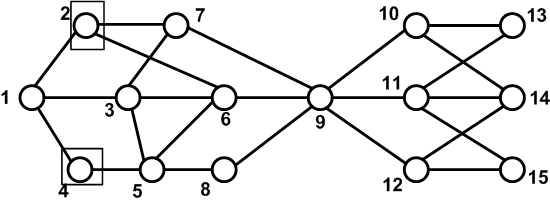
\includegraphics[width=0.5\textwidth]{./img/adversial_network.png}
\caption{Adverserial network}
\label{fig:adverserial_network}
\end{figure}

Other real-life applications of this concept include marketing -- promoting your product while a rival company is promoting a competing product -- or preventing the spread of misinformation. A recent example was the Kony 2012 campaign, a viral video spread by a non-profit activist organisation to highlight the issue of child soldiers in Uganda. The video spread very rapidly via online social networks; however, this soon led to people questioning the aims and methods of the campaigning organisation. This led to a counter-campaign that also spread virally, via social media. (Of course, which party provided misinformation in this scenario depends on individual perceptions).

[Limiting the Spread of Misinformation in Social Networks] looks more in depth at the problem of countering mis-information. They quantify this situation as a ``Multi-Campaign Independent Cascade Model'', where two campains, C and L, spread through a network. Each campaign has an initial seed set of nodes, A\_C/A\_L. As with the independent cascade model, when a node is converted, it has one chance to convert each of its neighbours. The probability that a node n converts its neighbour o is given by p\_C\_n\_o / p\_L\_n\_o, depending on which campaign the node was converted to. Note that in the general case, their may be different probabilities for the two campaigns (representing the situation where one campaign is more ``infectious'' than the other). Unlike in the independent cascade model, when an unconverted node has multiple converted neighbours, the order of ``conversion attempts'' matters; eg, campaign C may succeed in converting a node before campaign L has had the chance to convert it. Their model assumes that one campaign always precedes the other in such situations, ie, that campaign always gets the ``first chance''.

They also used a more specific model, the ``Campaign Oblivious Independent Cascade''. This is a special case of the multi-campaign model, where the conversion probabilities are the same for both campaigns.

They then look at minimising the influence of the opposing campaign, as opposed to maximising their own influence; this problem is referred to as the ``eventual influence limitation problem''. This can also be seen as maximising a function g(S), where S represents the seed set of campaign A (the ``good'' campaign), and g(S) computes the number of ``saved'' nodes -- ie, the number of nodes that were converted to campaign A, but would have been converted to campaign B if A was not present. Even with some simplifying assumptions (campaign B has a seed set consisting of only one node, campaign A has a conversion probability of 1), the problem is still NP-hard.

However, as with the two-state influence models, the function g can be shown to be submodular, and therefore a greedy algorithm can again achieve a performance of 1-(1/e) or ~63\%. This greedy algorithm works similarly to the one used for the influence maximisation problem; ie, iteratively adding to the seed set the node that will provide the best marginal improvement.

Although this is a polynomial-time algorithm, the datasets used for practical social network analysis may be extremely large, making even this algorithm unworkable in practice. Some alternative heuristics are therefore possible. These include the ``degree centrality heuristic'' (ie, choosing the nodes with the most incident edges), the ``early infectees heuristic'' (ie, choosing the nodes that are expected to be infected by the rival campaign early on), and the ``largest infectees heuristic'' (ie, choosing the nodes that are expected to infect the highest number of other nodes). By evaluating these heuristics via Monte Carlo simulations, it can be shown that the largest infectees heuristic is the most effective, approaching the performance of the greedy algorithm. The early infectees heuristic proved to be the least effective approach.




- Influence Maximisation Problem
-- limited budget of initially converted nodes
-- constrained optimisation problem
-- algorithm: non-negative, monotone, submodular
-- greedy algorithm

- attempt to find most influential nodes in a network

Cascading influence in blogs
http://cs.stanford.edu/people/jure/pubs/blogs-sdm07.pdf
- links between blogs
- 45k blogs and 2.2m posts
- is it bursty and/or periodic? does interest die off linearly or exponentially?
- popularity drops off in a power law
- size distribution of cascades follows a Zipfian distribution
- human networks tend to follow a power law distribution
- analyses cascade shapes

What stops social epidemics?
- existence of ``epidemic threshold'', critical value of transmissability
- large degree of heterogenity speeds up epidemics (Superspreading and the effect of individual variation on disease emergence.)

Digg
- spread of interest (votes) for a story through a users' friends
- not epidemic, why? network structure, 
- no increased chance to convert with multiple converted neighbours (friend saturation model)
- scale free number of fans
- only one epidemic story, michael jackson
- decreasing cascade model

A simple model of global cascades on
random networks
``These phenomena are all examples of what economists call
information cascades (ref. 4; but which are herein called simply
cascades), during which individuals in a population exhibit
herd-like behavior because they are making decisions based on
the actions of other individuals rather than relying on their own
information about the problem.''



\section{Emergent Behaviour}

The purpose of this component of the project is to observe and
describe how networks converge and to look at how robust these
networks are in the presence of infiltrators.  More specifically,
we will be looking at networks which use a tag-based approach to
cooperation and the infiltrators will be self-interested agents
which do not follow the social norms of the network.  In our case,
these self-interested agents could be thought of as law-enforcement
individuals.  In general, the presence of self-interested agents
have a negative affect on the cooperation within such a network.
Therefore, we will look at methods to preserve the cooperation rates
in networks where self-interested agents are present.

\subsection{Existing Research}

We are extending the work of Griffiths and Luck (2010) on tag-based
cooperation in a network in the presence of self-interested agents.
This work employs an image-scoring mechanism, network rewiring, and
a learning-based approach to evolution.

The work by Griffiths and Luck extends previous work on tag-based
cooperation, especially Riolo, Cohen, and Axelrod (2001); and Hales
and Edmonds (?).

\subsection{RCA Tag-based Cooperation}

Tag-based cooperation was introduced (Riolo, Cohen and Axelrod,
2001) to observe the nature and method that cooperation in a network
emerges.

The cooperation approach described by RCA takes place in a population
of agents.  Each agent is assigned a single tag and a single tolerance
value.  Both the tag and tolerance are selected randomly from a
uniform distribution between 0 and 1.
The tag is a cultural artefact, a form of a public identifier.
The tolerance is used to determine the willingness of an agent to cooperate.

The approach described by RCA is generational.  Each generation is
divided into two phases: a donation phase and a reproduction phase.
The donation phase occurs first, which allows every agent to perform
a number of donations.  After the donation phase, the reproduction
phase allows agents to reproduce based on their relative success.

During the donation phase, each agent in the population is selected
to make a number of donations.  The number of donations each agent
is selected to make is known as the number of interactions pairings
per generation, P.  When an agent has been selected for donation,
they pick an agent at random to which they have the opportunity to
donate.  In the RCA approach, an agent will donate to the random
agent if the difference between the two agents' tags is less than
the tolerance of the donator.  If an agent chooses to donate, they
will incur a small cost, c, and provide a benefit, b, to the receiving
agent.

\begin{align*}
    |\tau_A - \tau_B| < T_A
\end{align*}

The cooperation of a population of agents is measured by the donation rate in each generation.

Once every agent has been given an opportunity to donate $P$ times,
the reproduction phase takes place.  During the reproduction phase,
each agent reproduces in accordance with their relative success.
The most successful agents produce more offspring than the less
successful agents.  Each agent compares itself to a random agent.
If the agent is less successful than the random agent, then its
offspring derives from the random agent.  If the agent is more
successful than the random agent, then its offspring derives from
iteself.  The offspring takes the tag and tolerance values of the
more successful agent.  There is a small chance that the tag and
tolerance values could be mutated.  If the tag is mutated, the
offspring will receive a new tag taken randomly from the uniform
distribution $\left[0, 1\right]$.  If the tolerance is mutated, a
small amount of gaussian noise with a mean of $0$ is added to the
tolerance value.

Once the donation and reproduction phases for a given generation
have occurred, the process is repeated on the new population.

RCA noted that the donation rate quickly stabilises after around
100 generations.  Occasionally, an agent gets a tolerance value
that is much smaller than the average tolerance as the result of a
mutation.  This mutation allows the agent to become more successful
as they are less likely to donate.  The impact of this reduces the
overall donation rate until the agents converge on the new tag---due
to the reproduction process---at which time the donation rate raises
and stabilises again.

By experimentation, RCA found that with a higher number of interaction
pairings in each generation, the donation rate and average tolerance
increases.  RCA also noted that when the cost of donating became
too high relative to the benefit of receiving a donation, the
donation rate dropped dramatically.  From these results, we will
choose the number of interaction pairings per generation, $P$, to
be at least $3$, the cost of donation to be $0.1$, and the benefit
of receiving a donation to be $1$.

\subsection{Learning-Interpretation of Reproduction}

Hales and Edmonds (2003) extended the notion of tag-based cooperation by RCA
by introducing the notion of a {\emph learning} interpretation instead of a {\emph reproduction} interpretation.

The learning interpretation differs from the {\emph reproduction} interpretation of RCA
in that offspring are not produced in the reproduction phase.
Instead, when an agent is comparing itself to a more successful agent,
they will adopt that agents' tags and tolerances.
This means that the population of agents remains the same,
just the tag and tolerances of an agent change over generations.
Hales and Edmonds showed that the cooperation was not altered by adopting this approach.

Hales and Edmonds also changed the notion of the tag so that
the tag represented the neighbourhood of an agent.
When a new tag is learnt from another agent or through mutation,
the agent in effect rewires its neighbourhood to remove connections to those agents with its old tag,
and forging connections to agents with the same new tag.
In Hales and Edmonds' approach, donations are only permitted between agents in the same neighbourhood.

\subsection{Image Scoring}

Griffiths (2008) extended the cooperation approach of RCA,
using the learning interpretation of HE, by connecting agents
in a graph.
All agents are connected in a graph with a random network topology.
Agents are only able to donate to agents to which they are connected.

This model was used to observe the effect of self-interested agents (cheaters)
on the donation rate.
A cheater is an agent that never chooses to donate, despite the tags and tolerance values.
As such, a cheater is likely to be very successful as they
receive the benefits of donation without incurring the costs.
It was shown that the presence of just a small amount of cheaters in the network
caused a large reduction in the overall rates of cooperation.

To address this problem, image scoring was introduced.
In image scoring, each agent can observe the interation pairings of its neighbours.
Therefore,
and agent can keep track of the times when a neighbour chooses to donate and refuses to donate.
These observations for each neighbour are stored in a queue data structure.
When an agent is selected to make a donation, they will consider the observations of their local network
when donating in addition to their tag and tolerance values.

This approach to ranking a neighbourhood is chosen
due to the lack of direct reciprocity.
Direct reciprocity is when, by donating to another agent, it is likely that the other agent will in future donate to you.
It is therefore important to consider the neighbourhood to which an agent belongs when they make a donation.

\begin{align*}
    T_A' = T_A + \left(T_A \times \frac{\sum_{i = 1}^{n}\delta_i}{n}\right)
\end{align*}

Until each agent has recorded enough observations,
the basic tag and tolerance approach described by RCA is used.

It was observed that using this approach,
a significant increase in the donation rate, particularly
with small percentage of cheaters, could be achieved.

\subsection{Network Rewiring}

In order to further increase cooperation
in the presence of cheaters, network rewiring was introduced (Griffiths and Luck, 2010).
This allows an agent to rewire their connections to other agents,
in effect changing the neighbourhood of an agent.
The purpose of this is to allow an agent to remove connections
to agents which are unlikely to donate and forge connections to agents
which are more likely to donate.

Each agent which learnt during the learning phase,
is given an opportunity to rewire their own connections.
At this point, each of these agents is allowed to drop any number of its
connections to other agents and then add connections to new neighbours.
The aim of this is to allow agents to remove un-cooperative agents from
their neighbourhood in order to increase cooperation in their network.

There are two parameters that are used to control the rewiring phase:
the rewire proportion and the rewire strategy.
The rewire proportion is a percentage which is used to determine the number of
neighbours removed or added during a rewiring.
Whent the rewire proportion is zero, then no rewiring takes place.
When the rewire proportion is one, then all of an agents connections will be dropped and replaced with new connections.
There is a single rewire proportion value for all agents, which remains constant throughout the whole simulation.

The rewiring strategies determine which of an agents' connections are dropped and which new connections are to be acquired.
In their paper, Griffiths and Luck introduced four different rewiring strategies,
these are: Random, Random Replace Worst, Individual Replace Worst and Group Replace Worst.
For the purposes of the following descriptions of these strategies,
it is assumed that each neighbour of an agent can be ranked in order of their observed past donation behaviour.
This assumption is used to allow a rewiring strategy to identify the most and least cooperative agents in an agent's network.

\begin{description}
\item[Random Rewiring Strategy]
When the random rewiring strategy is used,
each agent will drop a proportion of their connections at random.
Once an agent has dropped these connections, the agent will then add new
connections to new agents at random to replace the connections dropped.

\item[Random Replace Worst Rewiring Strategy]
In this strategy, each agent will rank their neighbouring agents in terms
of their perceived willingness to donate, based on past observations.
Based on these rankings, the rewiring agent will drop their neighbours
which have the worst donation rate track record. Once these connections have
been dropped, random connections to new neighbours will be forged---as in
the random rewiring strategy.

\item[Individual Replace Worst Rewiring Strategy]
The individual replace worst strategy will---like the random replace
worst rewire strategy---remove connections to their neighbours which have
the worst record of donations. After these connections have been dropped,
the agent will look at their most willing neighbour and replace the lost
connections with their neighbour's best ranked connections. In the case where
adding a new connection would duplicate an existing connection, or connect an
agent to itself, a random connection is added instead. The effect of this is
that the new connections are the same as the best connections of their best
neighbour.

\item[Group Replace Worst Rewiring Strategy]
The group replace worst rewiring strategy is very similar to the individual
replace worst rewiring strategy. Like the individual replace worst rewiring
strategy, the neighbouring agents with the worst donation track record are
dropped. Once these connections have been dropped, the agent will connect
to the best ranked neighbour of each of its best ranked neighbours. As in the
individual replace worst rewiring strategy, any possible duplicate connections
will instead by replace by a random new connection.

\end{description}

\subsection{Effects of Rewiring Strategy on Cooperation}

To observe the effect of these different rewiring strategies as well as the
rewire proportion on the donation rate, Griffiths and Luck performed a number
of experiments.

It was found that the random rewiring strategy performed better than the RCA
approach, but worse than the RCA approach augmented with context assessment
(Griffiths, 2008). It was found that all the other rewiring strategies resulted
in a better donation rate than either of the RCA approaches. It was found that
rewiring was poorest when the rewiring proportion was close to zero or one.
It was found that the random replace worst rewwiring strategy performed poorly
when the rewiring proportion was greater than around $0.6$. It was found that
the individual and group replace worst rewiring strategies performed similarly
and had the best results when the rewire proportion was between $0.4$ and $0.8$.

From the results, it was show that by implementing these simple rewiring
strategies, it is possible to get a significant increase in overall cooperation---
in the paper, there was an increase of around 20\% over the image-scoring approach
in populations with 10\%, 20\%, and 30\% cheaters.

From these results, it appears to be sensible to choose a rewire proportion in
the range $0.4$ to $0.8$. In the paper, it was suggested to use a value of $0.6$
for the rewire proportion.


\section{Distributed Computing}
With the huge sizes social networks can reach, there needs to be efficient approaches to decrease the running time of algorithms for analysis of the networks. One approach is to use distributed computing to parallelise these algorithms, so that computation across the network occurs at the same time, where possible, and as such should reduce the running time of these algorithms.

One area of distributed computing which has been growing in recently is the use of the MapReduce framework developed by Google, and the free implementation by Apache of MapReduce, Hadoop. We will be looking to use Hadoop as an approach to parallelise algorithms for social network analysis.

This should achieve a reduced running time for algorithms, and also allow analysis of far larger networks than previously possible due to the scalability of the Hadoop framework.

\subsection{MapReduce}
MapReduce is a programming framework designed to simply processing data on large clusters \cite{mapreduce}. MapReduce works by the user supplying two functions, Map and Reduce, which operate in parallel on the data set provided. The Map function processes data from key/value pairs into an intermediate set of key/value pairs, before the Reduce function processes this intermediate set into final key/value pairs.

\lstset{language=C++,caption={Calculating the frequency of words in files using MapReduce \cite{mapreduce}},label=lst:mapreduceexample,tabsize=2,breaklines=true,breakatwhitespace=true,frame=single}
\begin{lstlisting}[float]
map(String key, String value):
	// key: document name
	// value: document contents
	for each word w in value:
		EmitIntermediate(w, ``1'');
		
reduce(String key, Iterator values):
	// key: a word
	// values: a list of counts
	int result = 0;
	for each v in values:
		result += ParseInt(v);
	Emit(AsString(result));	
\end{lstlisting}

Listing \ref{lst:mapreduceexample} is an example MapReduce program which counts the frequency of words within a selection of documents stored on a system. The Map function reads each word, \emph{w}, and emits the word as key/value pair \verb/(w, ``1'')/ to signify that there is an occurrence of \emph{w} at that position. The Reduce function sums together the value each of these emitted key/value pairs, where the key is the same, and emits the sum for each word.

Whilst the example given in Listing \ref{lst:mapreduceexample} uses Strings for the input and output for both of the Map and Reduce functions, it is not necessarily the case that all Map and Reduce functions operate in this way. \cite{mapreduce} explains that the types used by both are linked, as shown by:

\begin{verbatim}
map     (k1, v1)        -> list(k2, v2)
reduce  (k2, list(v2))  -> list(v2)
\end{verbatim}

This states the input keys and values are from a different domain to the output keys and values, which also means that the types used can differ.

MapReduce operates in two phases: The Map phase and the Reduce phase. Initially, the input data is split into small chunks to be assigned to the map tasks. A single map task is designated the master, with the remaining tasks designated as workers. The master assigns each map task a chunk of the input data to process, and once this has been processed, it is assigned more until all the input data has been processed. Once data from a map task has been processed, available reduce tasks then process this into the output data from the MapReduce program.

The MapReduce framework is highly fault tolerant, and is able to cope with multiple worker failure and failure of the master program as well. Each worker is required to periodically communicate with the master, and if no communication is received, then the worker is marked as failed, and its work is redistributed back out to be processed again. In case of the master failing, checkpoints are made and the MapReduce program can restart from the last checkpoint recorded.

\subsubsection{Google File System}
The Google File System, GFS, provides the distributed file system which MapReduce operates with \cite{mapreduce}, but was developed outside of MapReduce to address issues found with previous distributed file systems \cite{gfs}.

The GFS was designed to meet three major points identified with existing distributed file systems \cite{gfs}:
\begin{enumerate}
	\item Component failures are the norm, rather than the exception
	\item Files are huge by traditional standards
	\item Files are mutated by appending new data
\end{enumerate}

As hardware failures are common, the design of the GFS incorporates this, and the system is monitoring itself continually to detect, tolerate, and recover promptly from component failures on a routine basis \cite{gfs}. In addition to this, the system used by Google makes use of inexpensive hardware due to the frequent failures experienced, and as such is a more cost-effective solution than using more expensive tailored hardware.

A GFS cluster is split into a single $master$ and multiple $chunkservers$ and is accessed by multiple $clients$ \cite{gfs}. Files stored in the GFS are split into chunks, which are stored across the cluster on the hard disks located on each chunkserver. By default, each chunk is replicated in the file system three times for reliability of access to data within file system.

Files are stored into the GFS in chunks of size 64MB. This size was chosen to reduce the need to interact with master to find the location of chunks to read data from, and write data to. The larger chunk size also reduces the quantity of metadata stored on the master, which increases the performance of the master as the metadata can be stored in memory, reducing lookup times \cite{gfs}.

The master node maintains the metadata for the file system. This includes the locations of chunks across the file system, and which chunks compose the files stored. The master node communicates with each chunkserver frequently, and if it does not receive a response, the chunkserver is deemed to have failed and any chunks which are then under replicated in the file system are re-replicated to ensure that the minimum number of replications for each chunk are observed.

\subsection{Hadoop}
Hadoop\footnote{\url{http://hadoop.apache.org/}} is framework for performing
distributed computing. It is a free implementation of the MapReduce framework
developed at Google, and is also a top-level project hosted by Apache.

Hadoop has diversified itself from its conception, and is now composed of three
subprojects, Hadoop Common, Haddop Distributed File System, and Hadoop
MapReduce. Hadoop Common providse common utilities which support the other
Hadoop subprojects. The Hadoop Distributed File System is described in more
detail in Section \ref{sec:hdfs}

Hadoop MapReduce is the subproject by which Hadoop itself more known for. It
provides functionality similar to the MapReduce framework developed by Google,
where there exists a $Map$ and a $Reduce$ function which process data across a
cluster.

\subsubsection{Hadoop Distributed File System}
\label{sec:hdfs}
Hadoop also provides a the Hadoop Distributed File System, HDFS. The HDFS is a free implementation of the Google File System, and is designed to be used with Hadoop itself, though can also be used a distributed file system by itself \cite{hdfs}.

The HDFS operates in a similar approach to the operation of Hadoop and the Google File System. There exists a master node, called the NameNode, and many slave nodes, called DataNodes. The NameNode co-ordinates the access of files stored in the HDFS, and also manages the file system namespace. There is usually a DataNode present on each physical node within the cluster. It is the DataNode which control the storage of files on the storage system present on the node, and also controls the reading and writing of files to the HDFS from a user.

The HDFS ensures data integrity through replication of data across different nodes within the cluster. A replication factor is set for the cluster, generally at least 3, which causes all data within the HDFS to be replicated at least that many times. Data within the HDFS is split into blocks, with a large file being represented by many smaller blocks, and it is these blocks which are replicated across the HDFS.

In case of a problem with the HDFS, such as a partial network failure, or hard disk failure, each DataNode is required to periodically message the NameNode which contains a report on all data blocks stored by that DataNode. If there is a failure of some kind, then the NameNode either receives an incomplete message or no message at all. This informs the NameNode that there is a problem with the HDFS and takes appropriate action, including re-replicating the lost data from other DataNodes to new DataNodes.

The HDFS also provides another service called the SecondaryNameNode. The SecondaryNameNode is not a direct failover service to the NameNode. Instead, the SecondaryNameNode takes periodic checkpoints of the state of the NameNode, so that in case of the NameNode failing, a recent copy of the state of the HDFS can be loaded when the NameNode is restarted, which should result in minimal problems with resuming the HDFS.
\subsection{Graph Processing}
Whilst MapReduce and Hadoop provide a way for most algorithms to perform in a distributed manner, not all algorithms can be expressed in the MapReduce paradigm easily, or suffer from problems of being adapted to MapReduce when a different paradigm would be more suited. Google developed a framework called Pregel \cite{pregel}, and an open-source development inspired by Pregel, called Giraph \citep{giraphtalk} began in \citeyear{giraphtalk}

\subsubsection{Pregel}
Pregel is a framework developed at Google for large-scale graph processing. The purpose of Pregel was to produce a scalable and fault-tolerant platform with an API that is sufficiently flexible to express arbitrary graph algorithms \cite{pregel}. Existing solutions, other than Pregel, which achieve large-scale graph processing do suffer from issues ranging from poor performance, to a lack of fault tolerance within the system. Pregel addresses these issues within its framework.

A Pregel program executes as a series of parallel supersteps, similar in style to the Bulk Synchronous Parallel computation model described in \cite{bsp}. At each superstep, each active vertex performs some computation, which could modify the state of itself, its outgoing edges or send messages to other vertices to be received in the next superstep. An active vertex can also \emph{VoteToHalt}, which stops this vertex it from performing any extra computation whilst the algorithm is being executed, unless the inactive vertex receives a message, in which case it becomes active again to process the messages it has received. When all vertices have voted to halt, the algorithm terminates.

\begin{figure}[htbp]
  \centering
    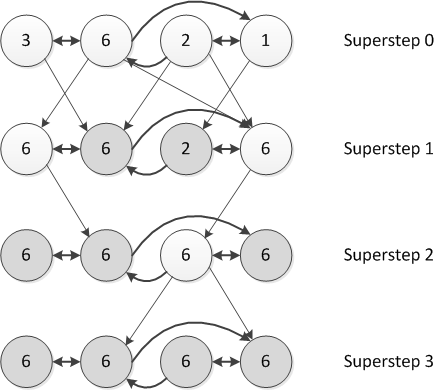
\includegraphics[width=0.5\textwidth]{./img/superstep}
  \caption{Maximum Value Example. Lighter lines are messages. Shaded vertices have voted to halt \cite{pregel}.}
  \label{fig:superstep}
\end{figure}

Figure \ref{fig:superstep} shows an example program in Pregel, which finds the maximum vertex value. Initially, all vertices are active, and send a message to each vertex they are connected directly containing their value. In the next superstep, if a vertex receives a message with a higher value than its currently stored value, then it stores the new higher value, otherwise the vertex deactivates as it currently has a local maximum whilst the program has not terminated. The vertices which did change send their value send a message containing their updated value to their neighbours. In superstep 2, the third vertex activates and changes its value from 2 to 6 as it receives a message containing the value 6. The two active vertices deactivate because they did not receive a message. The third vertex then sends a message to the second and fourth vertices containing the value 6, and in the third superstep, no vertex receiving a message changes its value, so does not need to send a message resulting in all vertices becoming inactive and terminating the program. The maximum value of all the vertices within the graph is now stored in all vertices.

As a Pregel program begins execution, multiple copies of the program start executing on a cluster of machines. A single copy is assigned as the \emph{master} which does not perform any work for the actual program, and instead manages the remaining \emph{worker} copies of the program. The \emph{master} partitions the input graph across the \emph{workers} and instructs the \emph{workers} to perform a superstep. This causes one iteration of the program to occur, and is repeated until all vertices vote-to-halt. The \emph{master} can the instruct each \emph{worker} to save its partition of the graph to memory.

The use of an underlying Bulk Synchonous Parallel model provides the Pregel framework with a simple way to model iteration of graph algorithms, and also provides a simple way to achieve a fault tolerant system. Each superstep in the execution of a Pregel program provides a natural barrier to synchronise each vertex's computation. If a \emph{worker} fails to communicate with the \emph{master} within a defined time period, the \emph{master} assumes that the \emph{worker} has failed, and can restart the program from the checkpoint made at the previous superstep completion, re-partitioning the graph if the failed \emph{worker} is still unavailable.

The Pregel framework also provides some extra useful features called combiners and aggregators. A combiner groups together a series of messages from one vertex to another into a single message containing the result of an operation on these messages. This is to reduce the overhead incurred from sending many messages and then performing the same operation at the receiving vertex. An aggregator is a global data construct, which each vertex has access to its value at each superstep, and the value can be updated at the end of each superstep in time for the next superstep. Aggregators can be used to store information about a graph, such as the number of edges in the graph.

Pregel also supports mutations of the graph an algorithm is being executed on. There are two types of mutations, global and local. A global mutation includes the addition and removal of vertices, as these can affect more that just a single vertex. Global mutations are partially ordered, and the effects of these mutations are seen in the next superstep. A local mutation includes a single vertex adding or removing an edge to another vertex. As these only affect the vertex which is performing these mutations, they happen immediately without any conflicts.

\lstset{language=C++,caption={PageRank algorithm in Pregel \cite{pregel}},label=lst:pregelpagerank,tabsize=2,breaklines=true,breakatwhitespace=true,frame=single}
\begin{lstlisting}[float]
class PageRankVertex
			: public Vertex<double, void, double> {
	public :	
		virtual void Compute(MessageIterator* msgs) {
g			if (superstep() >= 1) {
				double sum = 0;
				for(; !msgs->Done(); msgs->Next())
					sum += msgs->Value();
				*MutableValue() = 0.15 / NumVertices() + 0.85 * sum;
			}
			
			if (superstep() < 30) {
				const int64 n = GetOutEdgeIterator().size();
				SendMessageToAllNeighbors(GetValue() / n);
			} else {
				VoteToHalt();
			}
		}
};					
\end{lstlisting} 

Listing \ref{lst:pregelpagerank} shows how the PageRank algorithm \cite{pagerank} can be written using the Pregel framework. It can clearly be seen how the algorithm works. Each vertex receives a series of messages which contain the PageRank for the vertex which sent the message. The sum of these PageRanks is then computed, and the damping factor applied, and the result is stored as the value of the vertex. This values is then divided by the number of outgoing edges from the vertex, and is then sent as a message to each of the vertices the vertex is connected to.

\subsubsection{Giraph}
\label{sec:res_giraph}
Giraph is a graph processing framework, inspired by Pregel, initially developed at Yahoo!. It has since become an Apache Incubator project\footnote{\url{http://incubator.apache.org/giraph/}}. Giraph is still under development, with more features being added and improved. There are a number of existing solutions to achieve large-scale graph processing, however these also have their own problems.

Graph algorithms can be executed as a sequence of map-reduce jobs in Hadoop, but this suffers from the overheads of repeatedly launching these jobs and the map-reduce model is not a good fit for graph algorithms. Pregel itself has problems in that it requires a separate computing infrastructure, and is also unavailable to non-Google employees. The Message Passage Interface can also be used for graph processing, however it lacks any form of fault tolerance and is consider too generic \cite{giraphtalk}.

\lstset{language=Java,caption={PageRank algorithm in Giraph \cite{giraphtalk}},label=lst:giraphpagerank,tabsize=2,breaklines=true,breakatwhitespace=true,frame=single}
\begin{lstlisting}[float]
public class SimplePageRankVertex extends HadoopVertex<LongWritable, DoubleWritable, FloatWritable, DoubleWritable> {

	public void compute(Iterator<DoubleWritable> msgIterator) {
		double sum = 0;
		
		while (msgIterator.hasNext()) {
			sum += msgIterator.next().get();
		}
		
		setVertexValue(new DoubleWritable((0.15f/getNumVertices()) + 0.85f * sum);
		
		if (getSuperstep() < 30) {
			long edges = getOutEdgeIterator().size();
			
			sendMsgToAllEdges(new DoubleWritable(getVertexValue().get() / edges));
		} else {
			voteToHalt();
		}
	}
}					
\end{lstlisting}

Listing \ref{lst:giraphpagerank} shows the PageRank algorithm \cite{pagerank} produced using Giraph. Strong comparisons can be seen between this, and the Pregel implementation in Listing \ref{lst:pregelpagerank}. Both Listings show that a vertex receives a series of messages, of which the values of each are summer together. A damping factor is then applied and the result stored as the value of the vertex, before this value divided by the number of outgoing edges is sent to each vertex this vertex is connected to.

Small differences can be seen, due to Giraph using Hadoop as an underlying component, such as the type system used in Giraph being composed from Java objects as opposed to primitive date types in Pregel.

There are advantages to Giraph being built on top of Hadoop. Hadoop is being used by a large number of organisations for educational and production uses\footnote{\url{http://wiki.apache.org/hadoop/PoweredBy}} with other organisations providing Hadoop services for users\footnote{\url{http://wiki.apache.org/hadoop/Distributions and Commercial Support}}. This means that Giraph can be deployed onto these clusters with minimal effort required. It also means that Giraph only suffers from Hadoop-based problems, such as the Hadoop namenode and jobtracker being single points of failure for a Hadoop cluster.

Being inspired by Pregel, Giraph also makes use of the Bulk Synchronous Parallel computation model \cite{bsp}. Again for similar reasons to Pregel, the Bulk Synchronous Parallel model provides natural barriers for checkpoints during the execution of programs, and programs can restart from a previous superstep in the case of any failure. Giraph also operates with one copy of the program being designated the \emph{master} and the remaining copies being designated as \emph{workers}. The \emph{master} co-ordinates the \emph{workers}, and also handles the distribution of the input data across the cluster. The \emph{workers} execute the \verb/compute()/ method for every vertex on the partition of data they receive.

Giraph operates as a Map-only job on Hadoop, with there being no Reduce stage. A Giraph job has its own InputFormat and OutputFormat classes which call the user defined Vertex versions of these classes to load the data into each of the \emph{worker} processes.

The basic construct of a Giraph program is similar in style to a Hadoop program. Table \ref{tab:hadoopgiraph} shows this similarity. The \verb/compute()/ method of Giraph is analogous to the \verb/map()/ method of Hadoop. The I, V, E and M represent datatypes to be chosen by the user for their own implementation of Vertex, where:

\begin{itemize}
	\item I $\rightarrow$ VertexId
	\item V $\rightarrow$ VertexValue
	\item E $\rightarrow$ EdgeValue
	\item M $\rightarrow$ MsgValue
\end{itemize}

\begin{table}%
\centering
\begin{tabular}{|m{7.25cm}|m{7.25cm}|} \hline
Hadoop & Giraph \\ \hline
\begin{verbatim}

public class Mapper<
    KEYIN,
    VALUEIN,
    KEYOUT,
    VALUEOUT> {
  void map(KEYIN key,
           VALUEIN value,
           Context context)
           throws IOException,
           InterruptedException;
}
\end{verbatim} &
\begin{verbatim}
public class Vertex<
    I extends WritableComparable,
    V extends Writable,
    E extends Writable,
    M extends Writable> {
  void compute(
    Iterator<M> msgIterator);
}
\end{verbatim} \\
\hline
\end{tabular}
\caption{Comparison between basic Hadoop and Giraph program construct \cite{giraphtalk}}
\label{tab:hadoopgiraph}
\end{table}

